% lualatex
\documentclass[a4paper, 10pt]{ltjsarticle}
\usepackage{geometry}
\usepackage[fleqn]{amsmath}
\usepackage{amssymb, mathtools}
\usepackage{bm}
\usepackage{titlesec}
\usepackage{listings}
\usepackage{color}
\usepackage{tikz}
\usepackage{luatexja-fontspec}

\geometry{left=25mm,right=25mm,top=25mm,bottom=30mm}
\setmonofont{Ricty}

\renewcommand{\prepartname}{課題}
\renewcommand{\postpartname}{}

\newcommand{\ora}[1]{\overrightarrow{#1}}

\titleformat*{\section}{\normalsize}
\renewcommand{\thesection}{\textbf{\arabic{section}.}}
\titleformat*{\subsection}{\normalsize}
\renewcommand{\thesubsection}{\textbf{\arabic{section}.\arabic{subsection}.}}

\newcommand{\homework}{\part{}\setcounter{section}{0}}
\newcommand{\question}[1]{\section{#1}}
\newcommand{\subquestion}[1]{\subsection{#1}}
\newcommand{\exercises}[3]{\noindent\textsf{◇演習#1.#2:}\quad#3}

\renewcommand{\labelenumi}{(\alph{enumi})}

\newcommand{\Figref}[1]{\figurename~\ref{#1}}
\newcommand{\Tblref}[1]{\tablename~\ref{#1}}
\newcommand{\Equref}[1]{式(\ref{#1})}
\newcommand{\Lstref}[1]{\lstlistingname~\ref{#1}}

\renewcommand{\lstlistingname}{リスト}
\lstset{
    language = C,
    basicstyle = \ttfamily\small,
    commentstyle = \ttfamily\small\color[gray]{0.3},
    keywordstyle = \ttfamily\bfseries\small,
    identifierstyle = \ttfamily\small,
    numberstyle = \ttfamily\small,
    numbers = left,
    frame = single,
    xrightmargin = 0\zw,
    xleftmargin = 2\zw,
    stepnumber = 1,
    numbersep = 1\zw,
    lineskip = -0.5ex,
	breaklines = true,
	tabsize = 4
}

\begin{document}

%%%%%%%%%%%%%%%%%%%%%%%%%%%%%%%%
%%% 自己評価Sの演習
%%%%%%%%%%%%%%%%%%%%%%%%%%%%%%%%

\noindent\textsf{\LARGE 自己評価Sの演習}
\vspace{\baselineskip}

%%%%%%%%%%%%%%%%%%%%%%%%%%%%%%%%
%%% 演習4
%%%%%%%%%%%%%%%%%%%%%%%%%%%%%%%%

\exercises{4}{拡大縮小するウィンドウ}{
	ウィンドウサイズを2倍にしたら,ウィンドウ中の図形が2倍に拡大されて見えるような
	リサイズコールバック関数を作成せよ.
	ただし,ウィンドウの縦横比が変化しても,描画される図形の縦横比が変わらないようにせよ.
	例えばウィンドウサイズが$300 \times 200$画素のときは,
	WCSの$(-1.5, -1.0) \sim (1.5, 1.0)$の範囲が描画され,ウィンドウサイズが
	$200 \times 400$画素のときは,
	WCSの$(-1.0, -2.0) \sim (1.0, 2.0)$の範囲が描画されるような変換を考えればよい.
}

\vspace{\baselineskip}

% 文章

作成したリサイズコールバック関数を\Lstref{lst:ex04}に示す.
この関数はワールド座標系の矩形領域(\texttt{WCS\_L},\texttt{WCS\_B})$\sim$(\texttt{WCS\_R},\texttt{WCS\_T})
ウィンドウにギリギリ収まるように表示する.
ワールド座標系の表示する領域を設定できるため,汎用性が高く他のプログラムに応用しやすくなっている.
縦に余裕があるときの描画例と横に余裕があるときの描画例を\Figref{fig:ex04}に示す.
灰色の線は表示したい領域を示している.
ウィンドウにギリギリ収まるように描画できていることがわかる.

\lstinputlisting[
	caption = リサイズコールバック関数(\texttt{resize}),
	label = lst:ex04,
	linerange = {30-33, 35-37, 39-58}
]{
	../../Exercises/ex04.c
}

\begin{figure}[htbp]
	\centering
	\begin{minipage}[b]{0.4\textwidth}
		\centering
		
\includegraphics[scale=0.3]{../../Exercises/data/ex04-1.png}\\
		{\small (a) \; 縦に余裕があるとき}
	\end{minipage}
	\begin{minipage}[b]{0.5\textwidth}
		\centering
		
\includegraphics[scale=0.3]{../../Exercises/data/ex04-2.png}\\
		{\small (b) \; 横に余裕があるとき}
	\end{minipage}
	\label{fig:ex04}
	\caption{ウィンドウサイズ別の描画例}
\end{figure}


\newpage

%%%%%%%%%%%%%%%%%%%%%%%%%%%%%%%%
%%% 課題
%%%%%%%%%%%%%%%%%%%%%%%%%%%%%%%%

\noindent\textsf{\LARGE 課題}

% 課題I
%%%%%%%%%%%%%%%%%%%%%%%%%%%%%%%%
%%% 課題I
%%%%%%%%%%%%%%%%%%%%%%%%%%%%%%%%

\homework

%%%%%%%%%%%%%%%%%%%%%%%%%%%%%%%%
%%% I-1
%%%%%%%%%%%%%%%%%%%%%%%%%%%%%%%%

\question{
	\textsf{プログラミングツールのツール:}
	BCCにはMAKEユーティリティの他,grepやtouchなどプログラム開発に行う際に役に立つ
	コマンドラインツールが含まれている.それぞれの機能や利用法について学習せよ.\\
}

\vspace{-\baselineskip}

% make

\subquestion{MAKEユーティリティ}

Makeは,プログラムのビルドを自動化するために用いられるツールである.
ビルド作業が複雑になるときに特に役に立つ.
例えば,複雑に関連したソースファイルなどをビルドするとき,
長いコマンドや複数のコマンドが必要になる.
Makeによりそれらを一つにまとめビルド作業を簡単化できる.
makeコマンドを使うためにMakefileを規則に従って作る必要がある.
コマンドは以下のように使用する.\cite{Make}

\begin{lstlisting}[tabsize=1, numberstyle=\color{white}]
	make target
\end{lstlisting}

\vspace{-\baselineskip}

% Grep

\subquestion{grep}

Grepはテキストファイルから指定されたパターン(文字列)を1つまたは複数検索する.
コマンドを使うときにオプションを指定することでアルファベットの大文字小文字の区別
などを設定できる.コマンドは以下のように使用する.\cite{Grep}

\begin{lstlisting}[tabsize=1, numberstyle=\color{white}]
	grep [option] pattern file
\end{lstlisting}

\vspace{-\baselineskip}

% touch

\subquestion{touch}

touchは指定したファイルのアクセス時間(atime)や修正時間(mtime)を
書き換える.作成時間(ctime)は書き換えない.
コマンドは以下のように使用する.\cite{touch}

\begin{lstlisting}[tabsize=1, numberstyle=\color{white}]
	touch [option] file
\end{lstlisting}

%%%%%%%%%%%%%%%%%%%%%%%%%%%%%%%%
%%% I-2
%%%%%%%%%%%%%%%%%%%%%%%%%%%%%%%%

\question{
	\textsf{C言語:}変数の「有効範囲(Scope)」,「記憶域期間(記憶寿命)」
	について学習し,一般的な(ローカル)変数とグローバル変数,
	スタティック変数の違いを整理せよ.\\
}

\vspace{-\baselineskip}

% 有効範囲(Scope)

\subquestion{有効範囲(Scope)}

「有効範囲(Scope)」には,ブロック内を有効範囲(ブロック有効範囲)とする場合と
ファイル内を有効範囲(ファイル有効範囲)とする場合がある.
ブロック内とは\texttt{\{\}}で囲まれた部分のことで,
ファイル内とはファイル全ての範囲のことである.\cite{isl}

% 記憶域期間(記憶寿命)

\subquestion{記憶域期間(記憶寿命)}

「記憶域期間(記憶寿命)」には,自動記憶域期間と静的記憶域期間がある.
自動記憶域期間とは\texttt{auto}
\footnote{\texttt{auto}は省略することができるので一般に明示はしない.}
を使用して宣言したオブジェクト(変数)が持つ記憶域期間のことで,
オブジェクトは宣言したブロックに入ったときから終了するまで生存する.
静的記憶域期間とは,ファイル有効範囲のオブジェクトか\texttt{static}
を使用して宣言したときにオブジェクトが持つ記憶域期間のことで,
プログラムの開始から終了するまで生存する.\cite{atmarkit}

\pagebreak

\subquestion{各変数の有効範囲と記憶域期間}

ローカル変数,グローバル変数,スタティック変数の
有効範囲と記憶域期間をまとめたものを\Tblref{tbl:variable}に示す.
\begin{table}[htb]
	\centering
	\caption{各変数の有効範囲と記憶域期間}
	\begin{tabular}{l|c|c} \hline\hline
		\multicolumn{1}{c|}{変数} & 有効範囲 & 記憶域期間 \\ \hline
		ローカル変数     & ブロック有効範囲 & 自動記憶域期間 \\
		グローバル変数   & ファイル有効範囲 & 静的記憶域期間 \\
		スタティック変数 & ブロック有効範囲 & 静的記憶域期間 \\ \hline
	\end{tabular}
	\label{tbl:variable}
\end{table}

%%%%%%%%%%%%%%%%%%%%%%%%%%%%%%%%
%%% I-3
%%%%%%%%%%%%%%%%%%%%%%%%%%%%%%%%

\question{
	テキストの図1,図2のような図形(星型正多角形)を描き,
	回転させるプログラムを作成せよ.\\
}

\vspace{-\baselineskip}

% 星型正多角形

\subquestion{星型正多角形}

星型正多角形とは,正多角形と同様に全ての辺の長さが等しく全ての内角の大きさが等しいが
正多角形とは異なり辺同士が交わり合っている図形である.
注意として六芒星\footnote{2つの正三角形が重なってできている図形.}
のような幾つかの正多角形に分解できるものは星型正多角形に含まれない.
つまり,星型正多角形は一筆書きで書くことができる.\cite{Star}

$n$本の辺からなり元の位置に戻るために$m$周する星型正多角形について
$m$は多角形の密度と呼ばれ,星型正多角形になるための条件は,
$n$と$m$の最大公約数が$1$かつ,$n > 2m$である.
外角の和は$m$周することから$2\pi m$となり,
外角は$2\pi m / n = 2\pi / (n/m)$
\footnote{正多角形の場合も$m=1$となることから,この式は使える.}
で求めることができる.
このことから正多角形を星型正多角形に拡張して,正$n/m$角形と呼ばれる.
また,シュレーフリ記号(Schläfli symbol)では$\{n/m\}$と表記される.

% プログラム

\subquestion{プログラム}

演習3で作成した正多角形を描画するプログラムを
書き換えて星型正多角形(正$n/m$角形)を描画するプログラムを作成する.
作成した星型正多角形を描画する関数(\texttt{dispStarPolygon})を
\Lstref{lst:hw1-3-1}に示す.この関数は順に$n$,$m$,$\theta$を引数としている.
$\theta$は基準となる角度で,値を変えることで星型正多角形を回転させることができる.
関数\texttt{dispStarPolygon}を使い正$n/m$角形を回転させるためのプログラムを
\Lstref{lst:hw1-3-2}に示す.
\Lstref{lst:hw1-3-2}は1,2行目で正7/3角形に設定していて,
テキストのリスト11のタイマーコルバック関数を用いて,
$100\;[\mathrm{ms}]$経つたびに\texttt{rotAng}を$\pi/180$増加させ回転させている.
このプログラムの出力結果を\Figref{fig:hw1-3}に示す.

\lstinputlisting[
	caption = 星型正多角形を描画する関数(\texttt{dispStarPolygon}),
	label = lst:hw1-3-1,
	linerange = {28-31, 33-33, 35-43}
]{
	../../Homework/1/hw1-3.c
}
\lstinputlisting[
	caption = 星型正多角形を回転させるプログラム(主要部),
	label = lst:hw1-3-2,
	linerange = {5-6, 13-16, 18-18, 20-21, 23-23, 25-26}
]{
	../../Homework/1/hw1-3.c
}

%%%%%%%%%%%%%%%%%%%%%%%%%%%%%%%%
%%% I-4
%%%%%%%%%%%%%%%%%%%%%%%%%%%%%%%%

\question{
	テキストの図3,図4のような図形(完全グラフ)を描き,
	回転させるプログラムを作成せよ.\\
}

\vspace{-\baselineskip}

% 完全グラフ

\subquestion{完全グラフ}

完全グラフとは任意の2頂点間に必ずグラフがあるグラフのことをいう.
頂点が$n$個の完全グラフを$K_{n}$と表記し,
辺の数は頂点の組み合わせの数になるので$n(n-1) / 2$となる.\cite{Complete}

% プログラム

\subquestion{プログラム}

頂点の数が$n$の完全グラフ($K_{n}$)を描画するプログラムを作成する.
作成した完全グラフを描画する関数(\texttt{dispCompleteGraph})を
\Lstref{lst:hw1-4-1}に示す.この関数は順に$n$,$\theta$を引数としている.
まず全ての頂点の座標を配列に格納し,その後全ての辺を描いている.
関数\texttt{dispCompleteGraph}を使い$K_{n}$を回転させるためのプログラムは
\Lstref{lst:hw1-3-2}の9行目の\Lstref{lst:hw1-4-2}に書き換えたものとなる.
$n = 7$としたとき出力結果を\Figref{fig:hw1-4}に示す.

\lstinputlisting[
	caption = 完全グラフを描画する関数(\texttt{dispCompleteGraph}),
	label = lst:hw1-4-1,
	linerange = {27-31, 33-39, 41-52}
]{
	../../Homework/1/hw1-4.c
}
\lstinputlisting[
	caption = 関数\texttt{dispCompleteGraph}の呼び出し部分,
	label = lst:hw1-4-2,
	linerange = {20-20}
]{
	../../Homework/1/hw1-4.c
}

% 3, 4の出力結果

\begin{figure}[htbp]
	\centering
	\begin{minipage}[b]{0.45\textwidth}
		\centering
		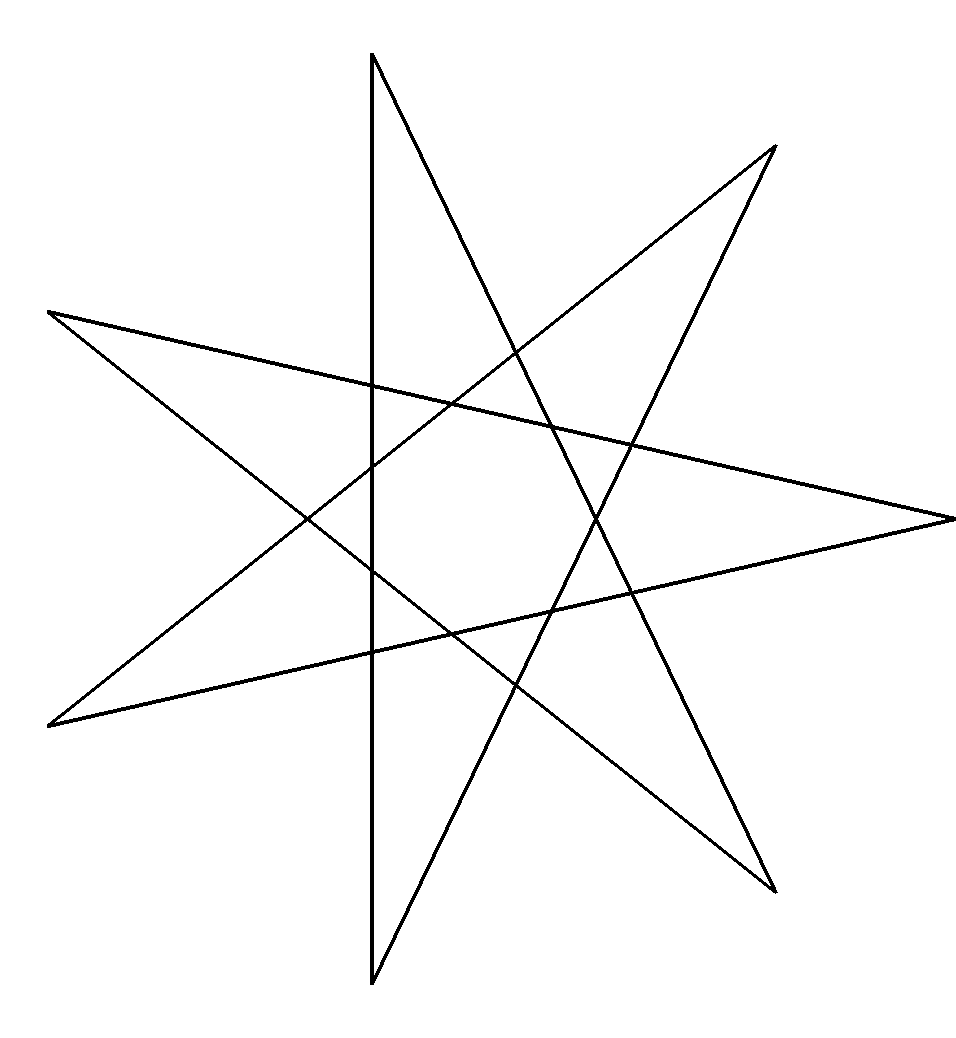
\includegraphics[scale=0.1]{../../Homework/1/data/hw1-3.png}
		\caption{正$7/3$角形の出力結果}
		\label{fig:hw1-3}
	\end{minipage}
	\begin{minipage}[b]{0.45\textwidth}
		\centering
		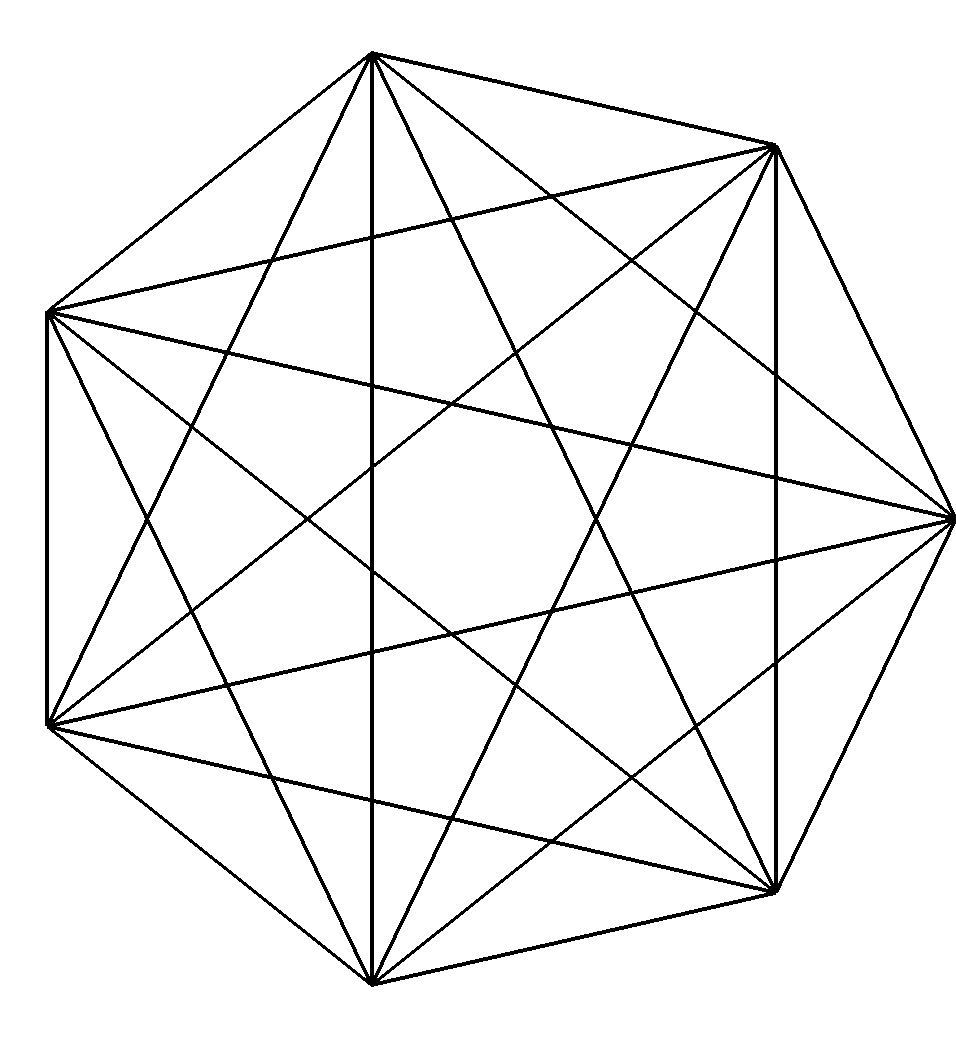
\includegraphics[scale=0.1]{../../Homework/1/data/hw1-4.png}
		\caption{$K_{7}$の出力結果}
		\label{fig:hw1-4}
	\end{minipage}
\end{figure}

%%%%%%%%%%%%%%%%%%%%%%%%%%%%%%%%
%%% I-5
%%%%%%%%%%%%%%%%%%%%%%%%%%%%%%%%

\question{
	テキストのリスト12を解析し,数学関数のグラフを描くプログラムを作成せよ.
	例えば$\theta$を$0$から$2\pi$まで変化させながら,次の関数をプロットすると
	どんな図形が描かれるだろうか(コラム参照).
	余力がある学生は,座標軸に目盛り(文字)を加えてみよ.
}

\begin{enumerate}
	\item カージオイド(cardioid)
	\begin{align}
		x &= [1 + \cos(\theta)]\cos(\theta)\label{equ:cardi-x}\\
		y &= [1 + \cos(\theta)]\sin(\theta)\label{equ:cardi-y}
	\end{align}
	\item サイクロイド(cycloid)
	\begin{align}
		x &= \theta - \sin(\theta)\label{equ:cycl-x}\\
		y &= 1 - \cos(\theta)\label{equ:cycl-y}
	\end{align}
	\item 4尖点の内サイクロイド(hypocycloid)
	\begin{align}
		x &= \cos^{3}(\theta)\label{equ:hypocycl-x}\\
		y &= \sin^{3}(\theta)\label{equ:hypocycl-y}
	\end{align}
\end{enumerate}

% プログラム

\subquestion{プログラム}

\Lstref{lst:hw1-5-1}にグラフを描画するために作成した関数のプロトタイプ宣言を示す.
関数\texttt{funcX},\texttt{funcY}に描くグラフの関数を設定する.
関数\texttt{setRange},\texttt{setXtics},\texttt{setYtics},\texttt{setRatio}は
グラフの設定パラメータを格納しているグローバル変数の書き換えをする関数で,
2つの軸の範囲,$x$軸の目盛り,$y$軸の目盛り,グラフの縦横比を設定する.
関数\texttt{dispGraph}はグラフを描くための関数で,関数内に目盛りを描くための
関数\texttt{drawXtics},\texttt{drawYtics}を使用する.
関数\texttt{dispGraph}を\Lstref{lst:hw1-5-2}に示す.
5から20行目でグラフの軸と目盛りを描画し,
22から28行目でグラフを描画している.
関数\texttt{setXtics},\texttt{setYtics}を\Lstref{lst:hw1-5-x},\Lstref{lst:hw1-5-y}に示す.
これらの関数はどちらも7から15行で$2l$の長さの目盛りを引いている.
17から29行目で,\texttt{setXtics}は表示する数字を目盛りの下になるようにして
\texttt{setYtics}は表示する数字を目盛りの左になるようにしている.

\lstinputlisting[
	caption = 関数のプロトタイプ宣言部分,
	label = lst:hw1-5-1,
	linerange = {9-17}
]{
	../../Homework/1/hw1-5.c
}
\lstinputlisting[
	caption = グラフ描画関数(\texttt{dispGraph}),
	label = lst:hw1-5-2,
	linerange = {32-60}
]{
	../../Homework/1/hw1-5.c
}
\lstinputlisting[
	caption = $x$軸の目盛り描画関数(\texttt{drawXtics}),
	label = lst:hw1-5-x,
	linerange = {62-91}
]{
	../../Homework/1/hw1-5.c
}
\lstinputlisting[
	caption = $y$軸の目盛り描画関数(\texttt{drawYtics}),
	label = lst:hw1-5-y,
	linerange = {93-122}
]{
	../../Homework/1/hw1-5.c
}

% 出力

\subquestion{各関数の出力結果}

この関数でカージオイド,サイクロイド,4尖点の内サイクロイドを
適切に軸の範囲や目盛りを設定して描画したグラフを
\Figref{fig:hw1-5-a},\Figref{fig:hw1-5-b},\Figref{fig:hw1-5-c}に示す.

\begin{figure}[htbp]
	\centering
	\begin{minipage}[b]{0.32\textwidth}
		\centering
		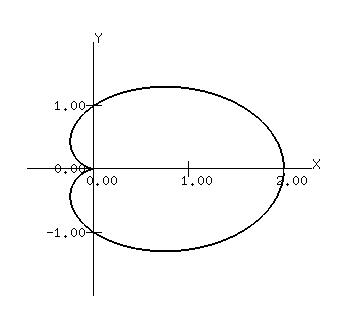
\includegraphics[scale=0.39]{../../Homework/1/data/hw1-5-a.png}
		\caption{カージオイド}
		\label{fig:hw1-5-a}
	\end{minipage}
	\begin{minipage}[b]{0.32\textwidth}
		\centering
		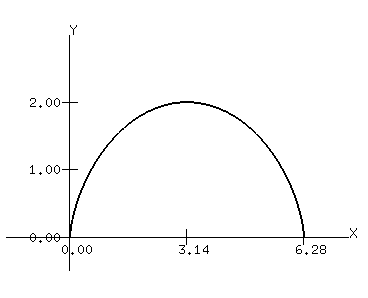
\includegraphics[scale=0.39]{../../Homework/1/data/hw1-5-b.png}
		\caption{サイクロイド}
		\label{fig:hw1-5-b}
	\end{minipage}
	\begin{minipage}[b]{0.32\textwidth}
		\centering
		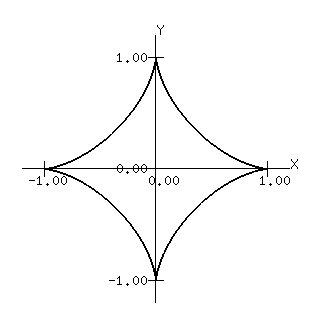
\includegraphics[scale=0.39]{../../Homework/1/data/hw1-5-c.png}
		\caption{4尖点の内サイクロイド}
		\label{fig:hw1-5-c}
	\end{minipage}
\end{figure}


% 課題II
%%%%%%%%%%%%%%%%%%%%%%%%%%%%%%%%
%%% 課題II
%%%%%%%%%%%%%%%%%%%%%%%%%%%%%%%%

\homework

%%%%%%%%%%%%%%%%%%%%%%%%%%%%%%%%
%%% II-1
%%%%%%%%%%%%%%%%%%%%%%%%%%%%%%%%

\question{
	テキストの図6に展開図を示す正四面体ABCD
	\footnote{本報告書では原点$\mathrm{O}$から$\bm{a}$にある点を$\mathrm{A}$と表記する.}
	について,$\triangle$BCDの重心Gを原点Oと一致させ,
	正四面体の一辺の長さを$w$とするとき,各頂点の3次元座標を導出せよ.
}

% 文章

$\triangle$BCDの高さは一辺が$w$の正三角形なので,$\sqrt{3}w/2$となる.
$\triangle$GBDが二等辺三角形となる.三平方の定理を用いて
$\triangle$GBDの等辺の長さは$w/\sqrt{3}$となる.
これらのことから正四面体の高さは三平方の定理を用いて,$\sqrt{2/3}w$となる.
よって各頂点の位置は次となる.
\begin{align*}
	\bm{a} &= \left(\sqrt{\frac{2}{3}}w, 0, 0\right) &
	\bm{b} &= \left(0, \frac{w}{\sqrt{3}}, 0\right) &
	\bm{c} &= \left(0, -\frac{w}{2\sqrt{3}}, \frac{w}{2}\right) &
	\bm{d} &= \left(0, -\frac{w}{2\sqrt{3}}, -\frac{w}{2}\right)
\end{align*}

% 図

\begin{figure}[htbp]
	\centering
	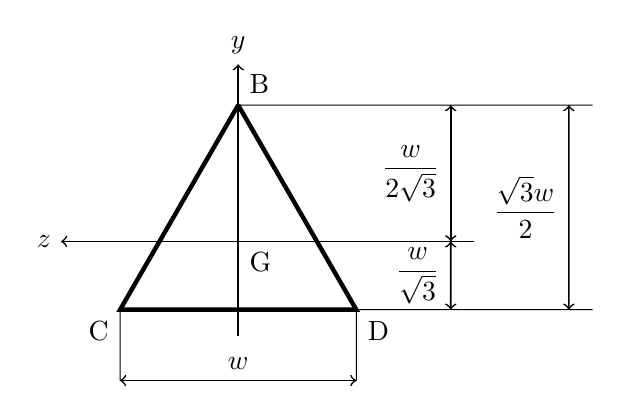
\begin{tikzpicture}[xscale=-3, yscale=3, ultra thick]
	%原点
	\draw (0, 0) node [below right]{G};
	%y軸
	\draw[semithick, ->] (0, -0.4)--(0, 0.75) node [above]{$y$};
	%z軸
	\draw[semithick, ->] (-1, 0)--(0.75, 0) node [left]{$z$};
	%頂点
	\path (0, 0.577) coordinate (B);
	\path (0.5, -0.289) coordinate (C);
	\path (-0.5, -0.289) coordinate (D);
	\draw (B) node [above right]{B};
	\draw (C) node [below left]{C};
	\draw (D) node [below right]{D};
	%辺
	\draw (B)--(C)--(D)--(B);
	%大きさ
	%
	\path (C)++(0, -0.3) coordinate (Cb);
	\draw[thin] (C)--(Cb);
	\path (D)++(0, -0.3) coordinate (Db);
	\draw[thin] (D)--(Db);
	\draw[semithick, <->] (Cb)--(Db);
	\draw (0, -0.589) node [above]{$w$};
	%
	\path (D)++(-0.4, 0) coordinate (Dr);
	\path (Dr)++(0, 0.289) coordinate (Or);
	\path (Dr)++(0, 0.866) coordinate (Br);
	\draw[semithick, <->] (Dr)--(Or);
	\draw[semithick, <->] (Or)--(Br);
	\path (Dr)++(0, 0.144) node [left]{$\displaystyle\frac{w}{\sqrt{3}}$};
	\path (Dr)++(0, 0.577) node [left]{$\displaystyle\frac{w}{2\sqrt{3}}$};
	%
	\path (D)++(-0.9, 0) coordinate (Drr);
	\path (Drr)++(0, 0.866) coordinate (Brr);
	\draw[semithick, <->] (Drr)--(Brr);
	\path (Drr)++(0, 0.433) node [left]{$\displaystyle\frac{\sqrt{3}w}{2}$};
	%
	\path (D)++(-1, 0) coordinate (Drrr);
	\path (Drrr)++(0, 0.866) coordinate (Brrr);
	\draw[thin] (D)--(Drrr);
	\draw[thin] (B)--(Brrr);
\end{tikzpicture}

	\hspace{4\zw}
	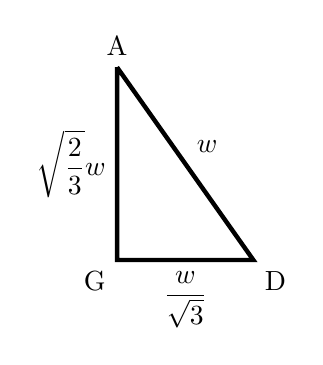
\begin{tikzpicture}[xscale=3, yscale=3, ultra thick]
	%頂点
	\path (0, 0.816) coordinate (A);
	\path (0, 0) coordinate (G);
	\path (0.577, 0) coordinate (D);
	\draw (A) node [above]{A};
	\draw (G) node [below left]{G};
	\draw (D) node [below right]{D};
	%辺
	\draw (A)--(G)--(D)--(A);
	%大きさ
	%
	\path (0, 0.408) node [left]{$\displaystyle\sqrt{\frac{2}{3}}w$};
	\path (0.289, 0) node [below]{$\displaystyle\frac{w}{\sqrt{3}}$};
	\path (0.289, 0.408) node [above right]{$\displaystyle w$};
\end{tikzpicture}

	\caption{正四面体の一部の大きさ}
	\label{fig:hw2-1}
\end{figure}

%%%%%%%%%%%%%%%%%%%%%%%%%%%%%%%%
%%% II-2
%%%%%%%%%%%%%%%%%%%%%%%%%%%%%%%%

\question{
	前問で求めた結果をもとに,原点Oを中心とする半径$1$の球に
	内接する正四面体の頂点がテキストのリスト14のように定まることを導出せよ.
}

% 文章

正四面体の重心$\bm{g}'$が原点と一致させるために前問の正四面体を移動させる.
重心$\bm{g}'$は,
\begin{align*}
	\bm{g}' = \frac{\bm{a} + \bm{b} + \bm{c} + \bm{d}}{4}
	= \left(\frac{1}{4}\sqrt{\frac{2}{3}}w, 0, 0\right)
\end{align*}
移動後の各頂点を$\bm{a}'$,$\bm{b}'$,$\bm{c}'$,$\bm{d}'$とすると各頂点の位置は,
\begin{align*}
	\bm{a}' &= \bm{a} - \bm{g}'
	= \left(\frac{1}{2}\sqrt{\frac{3}{2}}w, 0, 0\right) &
	\bm{b}' &= \bm{b} - \bm{g}'
	= \left(-\frac{1}{4}\sqrt{\frac{2}{3}}w, \frac{w}{\sqrt{3}}, 0\right)\\
	\bm{c}' &= \bm{c} - \bm{g}'
	= \left(-\frac{1}{4}\sqrt{\frac{2}{3}}w, -\frac{w}{2\sqrt{3}}, \frac{w}{2}\right) &
	\bm{d}' &= \bm{d} - \bm{g}'
	= \left(-\frac{1}{4}\sqrt{\frac{2}{3}}w, -\frac{w}{2\sqrt{3}}, -\frac{w}{2}\right)
\end{align*}
半径$1$の球に内接するとき$\bm{a}'=(1,0,0)$となるので$w=2\sqrt{2/3}$となる.
よって各頂点の位置は,
\begin{align*}
	\bm{a}' &= \left(1, 0, 0\right) &
	\bm{b}' &= \left(-\frac{1}{3}, \frac{2\sqrt{2}}{3}, 0\right) &
	\bm{c}' &= \left(-\frac{1}{3}, -\frac{\sqrt{2}}{3}, \frac{\sqrt{6}}{3}\right) &
	\bm{d}' &= \left(-\frac{1}{3}, -\frac{\sqrt{2}}{3}, -\frac{\sqrt{6}}{3}\right)
\end{align*}
この位置から各頂点の値がテキストのリスト14のように定まることがわかる.

%%%%%%%%%%%%%%%%%%%%%%%%%%%%%%%%
%%% II-3
%%%%%%%%%%%%%%%%%%%%%%%%%%%%%%%%

\question{
	テキストの\textbf{9.2}のアームロボットについて,キー入力で台座の回転と,
	各関節の傾斜角を制御できるような対話プログラムを作成してみよう.
}

% 文章

アームロボットの各パーツの登録部分を\Lstref{lst:hw2-3-1}に示す.
ここでは台座,下腕,上腕の登録をしている.
\footnote{
	\texttt{ID\_X}や\texttt{HEIGHT\_X}などは
	テキストのリスト27のようにマクロ定義してある.
}
キーボードコールバック関数を\Lstref{lst:hw2-3-2}に示す.
押されたキーに対応したパーツの角度を変え再描画している.
そして,テキストのリスト20と同様の関数\texttt{display}を用いて
アームロボットを描画する.

% リスト

\lstinputlisting[
	caption = 各パーツの登録(\texttt{init}の一部),
	label = lst:hw2-3-1,
	linerange = {14-14, 66-71, 73-81, 83-90, 92-100}
]{
	../../Homework/2/hw2-3.c
}
\lstinputlisting[
	caption = キーボードコールバック関数(\texttt{keyin}),
	label = lst:hw2-3-2,
	linerange = {13-13, 51-61, 63-65}
]{
	../../Homework/2/hw2-3.c
}

%%%%%%%%%%%%%%%%%%%%%%%%%%%%%%%%
%%% II-4
%%%%%%%%%%%%%%%%%%%%%%%%%%%%%%%%

\question{
	タイマーコールバックを使って,アームロボットを制御するようなプログラムを作成してみよう.
	アームロボットが踊っているかのように見せるには,どんな工夫ができるだろう.
}

% 踊ってるように見せるために

\subquestion{踊ってるように見せるために}

下腕と上腕を滑らかに手を振っているようにするには
各角度$\theta_{\mathrm{L}}$,$\theta_{\mathrm{U}}$を
\Equref{equ:theta-L},\Equref{equ:theta-U}とすることでできると考えた.(時刻を$t$とする.)
\begin{align}
	\theta_{\mathrm{L}} &= A\sin[B\sin(2t)]\label{equ:theta-L}\\
	\theta_{\mathrm{U}} &= A\sin[2B\sin(2t)]\;\;\;\;(AとBは任意定数)\label{equ:theta-U}
\end{align}
$A$と$B$を変えることで動きの速さを変えることができる.
下腕と上腕が揺れているところをいろいろな角度から見れるように,
台座を\Equref{equ:theta-B}で回転させる.
\begin{align}
	\theta_{\mathrm{B}} &= Ct\;\;\;\;(Cは任意定数)\label{equ:theta-B}
\end{align}

% プログラム

\subquestion{プログラム}

$A=45$,$B=1.5$,$C=5$に設定して
\Equref{equ:theta-L},\Equref{equ:theta-U},\Equref{equ:theta-B}
をタイマーコールバック関数に実装する.
作成したタイマーコールバック関数を\Lstref{lst:hw2-4-1}に示す.
これを全問のキーボードコールバック関数の代わりに使いアームロボットを踊らせる.

\lstinputlisting[
	caption = タイマーコールバック関数(\texttt{timer}),
	label = lst:hw2-4-1,
	linerange = {4-4, 17-17, 63-74}
]{
	../../Homework/2/hw2-4.c
}


% 課題III
%%%%%%%%%%%%%%%%%%%%%%%%%%%%%%%%
%%% 課題III
%%%%%%%%%%%%%%%%%%%%%%%%%%%%%%%%

\homework

%%%%%%%%%%%%%%%%%%%%%%%%%%%%%%%%
%%% III-1
%%%%%%%%%%%%%%%%%%%%%%%%%%%%%%%%

\question{
	空間中の任意の$3$点$\mathrm{P}_{i}(x_{i},y_{i},z_{i})$,$i=1,2,3$
	が与えられたとき,$\triangle\mathrm{P}_{1}\mathrm{P}_{2}\mathrm{P}_{3}$
	の単位法線ベクトルをすべて求める式を導出せよ.
}

$\triangle\mathrm{P}_{1}\mathrm{P}_{2}\mathrm{P}_{3}$を含む平面上の
互いに平行でない2つのベクトルの外積は,その平面の法線ベクトルになる.
ここで2つのベクトルを$\ora{\mathrm{P}_{1}\mathrm{P}_{2}}$と$\ora{\mathrm{P}_{1}\mathrm{P}_{3}}$
とすると,$\triangle\mathrm{P}_{1}\mathrm{P}_{2}\mathrm{P}_{3}$のすべての単位法線ベクトルは,
\begin{align*}
	\pm
	\frac{
		\ora{\mathrm{P}_{1}\mathrm{P}_{2}} \times \ora{\mathrm{P}_{1}\mathrm{P}_{3}}
	}{
		\left|\ora{\mathrm{P}_{1}\mathrm{P}_{2}} \times \ora{\mathrm{P}_{1}\mathrm{P}_{3}}\right|
	}
\end{align*}
となる.

%%%%%%%%%%%%%%%%%%%%%%%%%%%%%%%%
%%% III-2
%%%%%%%%%%%%%%%%%%%%%%%%%%%%%%%%

\question{
	空間中の任意の$3$点$\mathrm{P}_{i}(x_{i},y_{i},z_{i})$,$i=1,2,3$
	が与えられたとき,$\triangle\mathrm{P}_{1}\mathrm{P}_{2}\mathrm{P}_{3}$
	のどちらが表(CCW)で,どちらが裏(CW)と判定できるか,判定方法を導出せよ.
}

右手系の外積で,$\ora{\mathrm{P}_{1}\mathrm{P}_{2}} \times \ora{\mathrm{P}_{1}\mathrm{P}_{3}}$
が正となるとき表になる.負のとき裏になる.

%%%%%%%%%%%%%%%%%%%%%%%%%%%%%%%%
%%% III-3
%%%%%%%%%%%%%%%%%%%%%%%%%%%%%%%%

\question{
	Phongの照光モデルについて,詳しく調べよ.
}

% 発表

\subquestion{発表}

Phongの照光モデル\footnote{Phongの反射モデルとも呼ばれる.}
(Phong reflection model)は
ユタ大学の理学博士であるBui Tuong Phongによって開発され,1973年に学位論文\cite{Utah},
1975年に論文(Illumination for Computer Generated Pictures)\cite{Bui}として発表された.

% 概要

\subquestion{概要}

現実の光源では反射現象により物体に複数の方向からいろいろな光が当たる.
コンピュータ上でこれらを全て扱うことは非常に困難であるため,単純化を行う必要がある.
ここで反射現象を単純化するためにPhongの照光モデルを用いる.
このモデルは物体の表面からの反射光を
環境光の反射光\footnote{環境光は間接光とも呼ばれ,別の物体表面での反射を経て物体表面に届く光のこと.},
直接光の拡散反射光\footnote{拡散反射光は,反射角にほとんど依存せず多様な方向に反射した光のこと.},
直接光の鏡面反射光\footnote{鏡面反射光は反射角が入射角と等しくなるように反射した光のこと.}
の3つの反射光の和で近似する.

% 計算方法

\subquestion{計算方法}

物体表面の輝度を$L_{\mathrm{r}}$,環境光の反射光の輝度を$L_{\mathrm{a}}$,
直接光の拡散反射光の輝度を$L_{\mathrm{d}}$,直接光の鏡面反射光の輝度を$L_{\mathrm{s}}$とすると,
$L_{\mathrm{r}}$は\Equref{equ:L-r}となる.
\begin{align}
	L_{\mathrm{r}} = L_{\mathrm{a}} + L_{\mathrm{d}} + L_{\mathrm{s}}\label{equ:L-r}
\end{align}
環境光反射係数を$k_{\mathrm{a}}$,環境光の照度を$E_{\mathrm{a}}$とすると,
$L_{\mathrm{a}}$は\Equref{equ:L-a}となる.
\begin{align}
	L_{\mathrm{a}} = k_{\mathrm{a}}E_{\mathrm{a}}\label{equ:L-a}
\end{align}
拡散反射係数を$k_{\mathrm{d}}$,入射光の照度を$E_{\mathrm{i}}$,
物体表面の単位法線ベクトルを$\bm{n}$,光の入射方向の単位ベクトルを$\bm{l}$とすると,
$L_{\mathrm{d}}$は\Equref{equ:L-d}となる.
\begin{align}
	L_{\mathrm{d}} = k_{\mathrm{d}}E_{\mathrm{i}}(\bm{n}\cdot\bm{l})\label{equ:L-d}
\end{align}
鏡面反射係数を$k_{\mathrm{s}}$,入射光の照度を$E_{\mathrm{i}}$,
視線と逆向きの単位ベクトルを$\bm{v}$,入射光の正反射単位ベクトルを$\bm{r}$,
光沢度を$\alpha$とすると,$L_{\mathrm{s}}$は\Equref{equ:L-s}となる.
\begin{align}
	L_{\mathrm{s}} = k_{\mathrm{s}}E_{\mathrm{i}}(\bm{v}\cdot\bm{r})^{\alpha}\label{equ:L-s}
\end{align}
\Equref{equ:L-a},\Equref{equ:L-d},\Equref{equ:L-s}より\Equref{equ:L-r}は\Equref{equ:L}となる.
\begin{align}
	L_{\mathrm{r}}
	= k_{\mathrm{a}}E_{\mathrm{a}}
	+ k_{\mathrm{d}}E_{\mathrm{i}}(\bm{n}\cdot\bm{l})
	+ k_{\mathrm{s}}E_{\mathrm{i}}(\bm{v}\cdot\bm{r})^{\alpha}\label{equ:L}
\end{align}

%%%%%%%%%%%%%%%%%%%%%%%%%%%%%%%%
%%% III-4
%%%%%%%%%%%%%%%%%%%%%%%%%%%%%%%%

\question{
	正四面体,正六面体,正八面体をスムーズシェーディングで表示するために,
	各頂点の単位法線ベクトルをどのように定めればよいか考え,実装せよ.
}

% 頂点の単位法線ベクトル

\subquestion{頂点の単位法線ベクトル}

頂点の単位法線ベクトルは重心から頂点に向かうベクトルと同じ方向になる.
よって原点を中心とする半径1の球に内接する正多面体の頂点ベクトルが頂点の単位法線ベクトルとなる.

% プログラム

\subquestion{プログラム}

テキストのリスト21と演習19で求めた正四面体,正六面体,正八面体の頂点の座標を使い
各正多面体をスムーズシェーディングで表示するプログラムを作成する.
正四面体をスムーズシェーディングで表示するプログラムの主要部を\Lstref{lst:hw3-4-a}に示す.
\texttt{g\_vP}は頂点の座標,\texttt{g\_tp}はトポロジ情報を格納してある.
そして関数\texttt{display}で正四面体を表示している.
正六面体,正八面体をスムーズシェーディングで表示するプログラムの主要部を
\Lstref{lst:hw3-4-b},\Lstref{lst:hw3-4-c}に示す.これらも同様の処理で表示している.
スムーズシェーディングで表示された正多面体を\Figref{fig:hw3-4}に示す.
\footnote{光源はデフォルトの\texttt{GL\_LIGHT0}に設定してある.}

\lstinputlisting[
	caption = 正四面体をスムーズシェーディングで表示するプログラム(主要部),
	label = lst:hw3-4-a,
	linerange = {8-16, 18-21, 23-25, 32-41, 43-44}
]{
	../../Homework/3/hw3-4-a.c
}
\lstinputlisting[
	caption = 正六面体をスムーズシェーディングで表示するプログラム(主要部),
	label = lst:hw3-4-b,
	linerange = {8-21, 23-26, 28-30, 37-46, 48-49}
]{
	../../Homework/3/hw3-4-b.c
}
\lstinputlisting[
	caption = 正八面体をスムーズシェーディングで表示するプログラム(主要部),
	label = lst:hw3-4-c,
	linerange = {8-19, 21-24, 26-28, 35-44, 46-47}
]{
	../../Homework/3/hw3-4-c.c
}

\begin{figure}[htbp]
	\centering
	\begin{minipage}[b]{0.32\textwidth}
		\centering
		
\includegraphics[scale=0.23]{../../Homework/3/data/hw3-4-a.png}\\
		{\small (a) \; 正四面体}
	\end{minipage}
	\begin{minipage}[b]{0.32\textwidth}
		\centering
		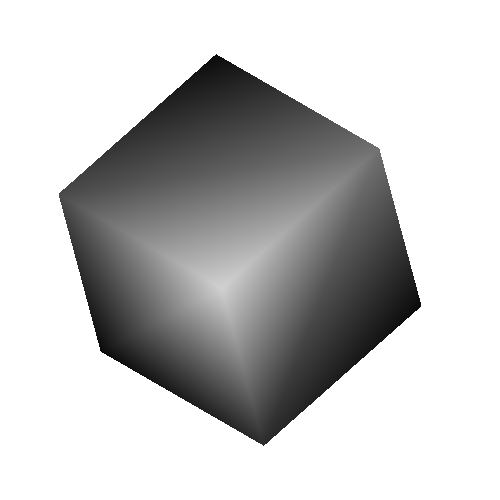
\includegraphics[scale=0.23]{../../Homework/3/data/hw3-4-b.png}\\
		{\small (b) \; 正六面体}
	\end{minipage}
	\begin{minipage}[b]{0.32\textwidth}
		\centering
		
\includegraphics[scale=0.23]{../../Homework/3/data/hw3-4-c.png}\\
		{\small (c) \; 正八面体}
	\end{minipage}
	\caption{スムーズシェーディングで表示された正多面体}
	\label{fig:hw3-4}
\end{figure}

%%%%%%%%%%%%%%%%%%%%%%%%%%%%%%%%
%%% III-5
%%%%%%%%%%%%%%%%%%%%%%%%%%%%%%%%

\question{
	テキストのリスト27を参考に,アームロボットをシェーディング表示
	するものに変更してみよ.
}

% 文章

各パーツの角度を格納する\texttt{g\_rotAng}をグローバル変数に定義する.
そして各パーツを描画する前に関数\texttt{glRotated}を用いて回転させる.
\texttt{g\_rotAng}の値を書き換えるために\Lstref{lst:hw2-3-2}のキーボードコールバック関数を用いた.
ソースコードの他の部分はテキストのリスト27と同様である.
描画されたアームロボットを\Figref{fig:hw3-5}に示す.

\lstinputlisting[
	caption = アームロボットをシェーディング表示するプログラム(主要部),
	label = lst:hw3-5,
	linerange = {35-35, 44-50, 52-53, 55-57, 59-61, 63-64}
]{
	../../Homework/3/hw3-5.c
}

\begin{figure}[htbp]
	\centering
	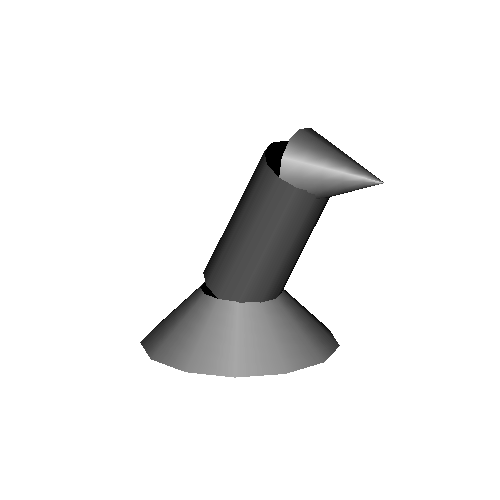
\includegraphics[scale=0.3]{../../Homework/3/data/hw3-5.png}\\
	\caption{シェーディング表示されたアームロボット}
	\label{fig:hw3-5}
\end{figure}


\newpage

%%%%%%%%%%%%%%%%%%%%%%%%%%%%%%%%
%%% 感想,改善案,参考文献
%%%%%%%%%%%%%%%%%%%%%%%%%%%%%%%%

\noindent{\textsf{\large 感想}}
\vspace{0.5\baselineskip}

課題で調べごとをするときに,できるだけ英語の文献を参考にするようにした.
本科目の目的とは関係ないが,英語の苦手意識を少しでも軽減できたり,
英語の文献の検索や読む練習になったりするので努力した.
また,日本語でまとめているサイトではなく公式のサイトを参考にする場合
しっかりとした情報が得られてよかった.
これから更に英語の文献に触れる機会が増えると思うので英語に慣れていきたい.
演習や課題の手応えはちょうどよくスムーズに進んでよかった.
受講して非常に良かった.(受講しない場合は研究室を破門されるが...)

\vspace{0.5\baselineskip}
\noindent{\textsf{\large 改善案}}
\vspace{0.5\baselineskip}

課題III-5はリストを写すだけなので演習にするべきだと思う.
関数\texttt{abc}や\texttt{abc}関数や\texttt{abc*}の表記の違いがわかりにくいです.
違いがないなら統一したほうが良いのではないでしょうか.

\renewcommand{\refname}{\large{\textsf{参考文献・URL}}}
\begin{thebibliography}{99}
	\bibitem{textbook}{
		高橋章,R01-Ec5 プログラミング演習IVテキスト
	}
	\bibitem{Make}{
		GNU Make,
		\texttt{http://www.gnu.org/software/make/}
	}
	\bibitem{Grep}{
		GNU Grep,
		\texttt{http://www.gnu.org/software/grep/}
	}
	\bibitem{touch}{
		touch,\\
		\texttt{http://www.gnu.org/software/coreutils/manual/html\_node/touch-invocation.html}
	}
	\bibitem{isl}{
		変数のスコープ,
		\texttt{http://www.isl.ne.jp/pcsp/beginC/C\_Language\_09.html}
	}
	\bibitem{atmarkit}{
		Cにおける識別子の有効範囲と変数の生存期間,\\
		\texttt{https://www.atmarkit.co.jp/ait/articles/1104/26/news107.html}
	}
	\bibitem{Star}{
		Star Polygon,
		\texttt{http://mathworld.wolfram.com/StarPolygon.html}
	}
	\bibitem{Complete}{
		Complete Graph,
		\texttt{http://mathworld.wolfram.com/CompleteGraph.html}
	}
	\bibitem{Utah}{
		University of Utah School of Computing,
		\texttt{https://www.cs.utah.edu/about/history/\#phong-ref}
	}
	\bibitem{Bui}{
		Illumination for Computer Generated Pictures,Bui Tuong Phong,\\
		\texttt{https://users.cs.northwestern.edu/\~{}ago820/cs395/Papers/Phong\_1975.pdf}
	}
	\bibitem{Phong}{
		Phongの反射モデル,
		\texttt{https://knzw.tech/raytracing/?page\_id=240}
	}
\end{thebibliography}

\end{document}
